\documentclass[a4paper]{report}   

\usepackage[utf8]{inputenc}
\usepackage[francais]{babel}

\usepackage{multirow}
\usepackage{graphicx}
\usepackage{amsmath}
\usepackage{hyperref}

\usepackage{cite}


\usepackage[french]{algorithm2e}

\usepackage{enumerate}

\title{Détection d'anomalies de classification dans l'IoT via Machine Learning}
\author{Antoine Urban, Yohan Chalier}
\date{\today}

\renewcommand{\arraystretch}{1.2}

\usepackage{etoolbox}
\apptocmd{\thebibliography}{\raggedright}{}{}

\begin{document}

\begin{titlepage}
	\centering
	\vspace{1cm}
	\begin{figure}
	\centering
	\includegraphics[scale=0.2]{img/logo_TPT.png}
	\end{figure}
	\vspace{1cm}
	{\scshape\LARGE Télécom ParisTech \par}
	\vspace{1cm}
	{\scshape\Large Projet de filière SR2I \par}
	\vspace{1.5cm}
	{\huge\bfseries Détection d'anomalies de classification dans l'IoT via Machine Learning\par}
	\vspace{2cm}
	{\Large\itshape Antoine Urban, Yohan Chalier \par}
	\vfill
	encadrés par\par
	Jean-Philippe \textsc{Monteuuis}\par
	Houda \textsc{Labiod}
	\vfill

% Bottom of the page
	{\large \today\par}
\end{titlepage}

\begin{abstract}
Dans le contexte de l'internet des objets, les messages peuvent contenir de fausses informations générées par un utilisateur authentifié. Par conséquence, les mécanismes de sécurité reposant sur le chiffrement et la signature des messages sont inefficaces face à ces attaques. Les classeurs basés reposant sur l'apprentissage machine (Machine Learning) permettent de classer si un objet émettant des données est malicieux ou non.
\end{abstract}

\chapter{Introduction}

L'exercice de la conduite est synonyme de changements constants. Ainsi, lorsque nous conduisons, notre attention est entièrement consacrée à notre environnement, car notre sécurité et celle des personnes qui nous entourent sont en jeu. Nous prêtons une attention particulière aux obstacles qui peuvent surgir, qu'il s'agisse tout simplement d'autres voitures partageant la route, des piétons ou encore des motocyclistes.

\begin{figure}
\centering
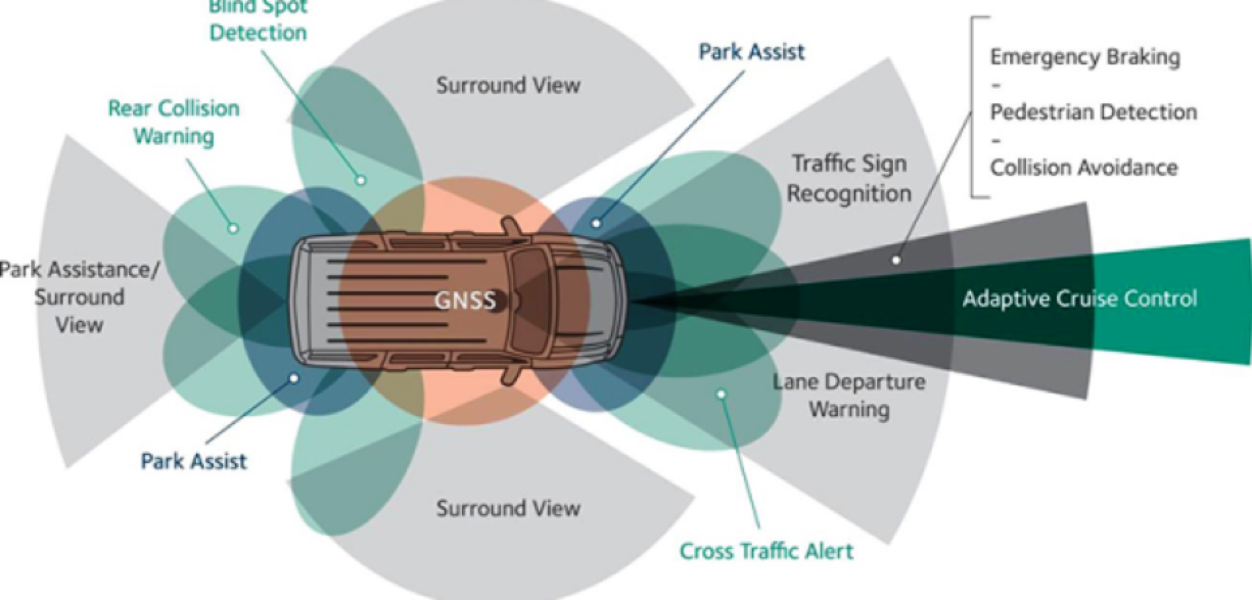
\includegraphics[width=\textwidth]{img/sensors.png}
\caption{Ensemble des capteurs présents dans le véhicule\label{sensors}}
\end{figure}

Longtemps fantasmés, les véhicules autonomes sont aujourd'hui réalité grâce aux incroyables progrès réalisés dans les domaines de l'intelligence artificielle et du développement de capteurs. Si ces processus visent à remplacer le conducteur humain, il semble naturel qu'ils prêtent la même attention aux obstacles. La Figure \ref{sensors} présente la complexité introduite dans ce nouvel environnement. Un nombre important de capteurs est en effet nécessaire pour avoir une vue complète du contexte extérieur. Cela comprend à la fois des communications Véhicule-à-Véhicule et l'analyse des données des capteurs.

~\par

Dans ce travail, nous nous concentrerons sur les trois types d'obstacles les plus communs sur une route :
\begin{itemize}
\item une voiture,
\item une moto et
\item un piéton.
\end{itemize}

~\par

Tout travail sur l'analyse d'obstacles nécessite la détection préalable de régions d'intérêt en utilisant par exemple la méthode du "point-in-polygon" \cite{ref1}, ou encore à l'aide de capteurs à ultrasons et d'analyse de signal \cite{ref2}. Ce travail n'a pas comme objectif de revenir sur l'utilisation de ces techniques, mais se concentrera sur l'analyse à posteriori des dimensions ainsi collectées avec pour but de proposer une classification efficace. La Figure \ref{data_flow} récapitule le flot de données dans un véhicule autonome. Comme nous pouvons le voir, en collectant les données des capteurs et provenant des véhicules aux alentours, le travail de classification (ou "perception") permet la modélisation de l'environnement et de déterminer le comportement du véhicule.

\begin{figure}
\centering
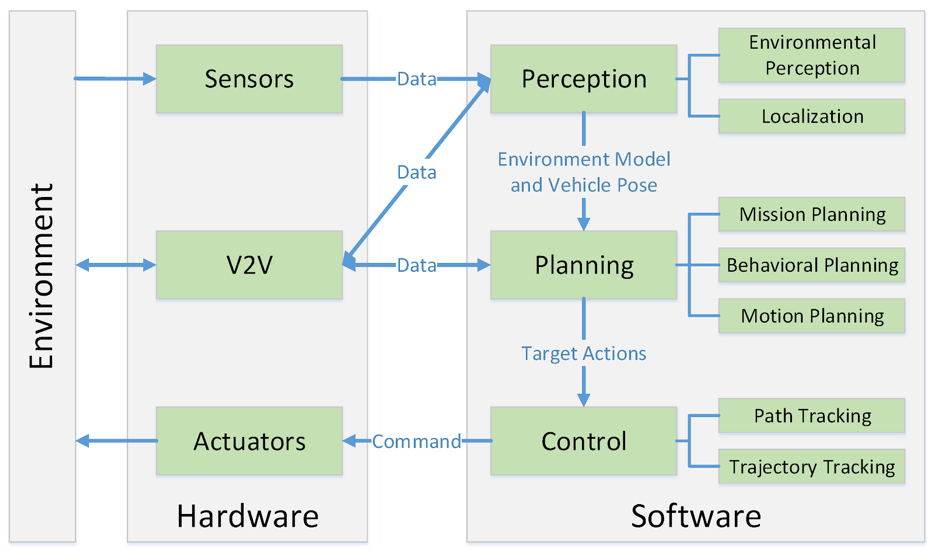
\includegraphics[width=\textwidth]{img/data_flow.png}
\caption{Flux de données\label{data_flow}}
\end{figure}

\section{Attaques}

Comme nous l'avons vu grâce aux figures \ref{sensors} et \ref{data_flow}, le nombre important de capteurs et la collecte de messages provenant de véhicules rendent la surface d'attaque importante. Cette section a pour objectif de décrire les plus importantes.

\begin{description}\setlength{\itemsep}{1.5mm}
\item[Attaque par aveuglement des capteurs] La présence de capteurs optiques rend possible une attaque par aveuglement. Dans ce schéma \cite{blinding}, un attaquant utilise un laser pour aveugler ces capteurs ce qui a pour conséquence une mauvaise perception de l'environnement. De ce fait, la victime pourra freiner ou dévier de sa trajectoire et ainsi provoquer un accident. 
\item[Attaque par modification] Un attaquant peut envoyer des faux messages à la victime. Cela aura pour conséquence de causer une fausse perception de l'environnement et incidemment créer un accident.
\end{description}

\begin{figure}
\centering
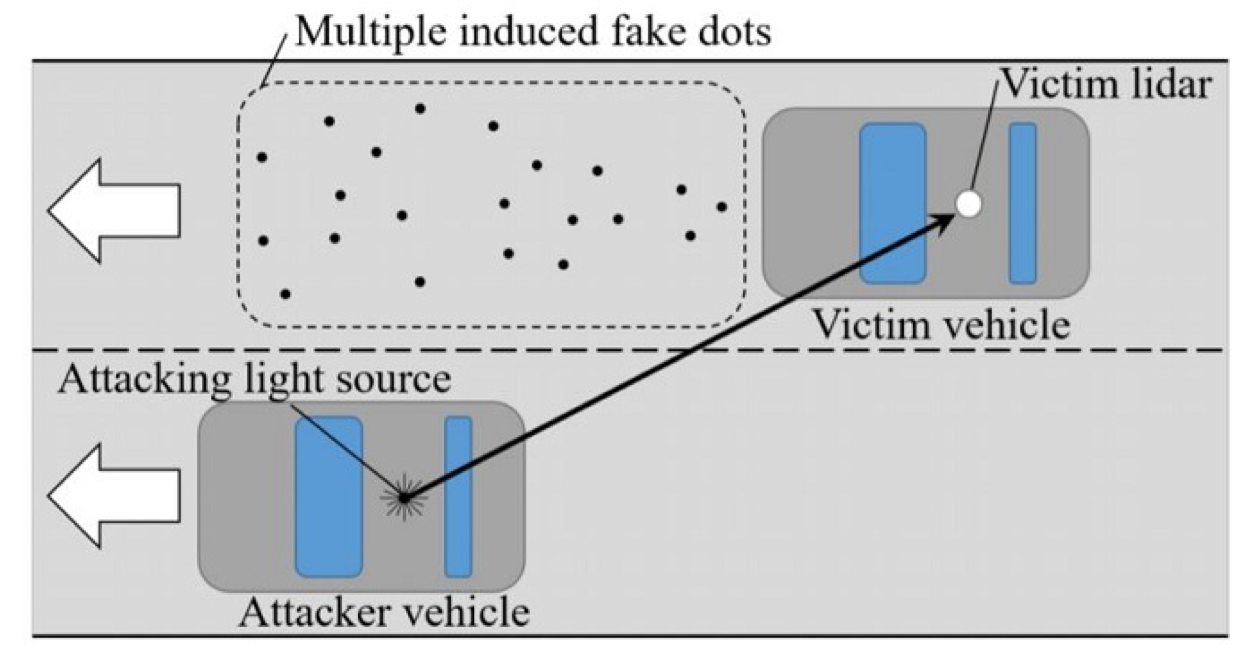
\includegraphics[width=\textwidth]{img/blinding.png}
\caption{Attaque par aveuglement\label{blinding}}
\end{figure}

\section{Travaux connexes}

Le sujet de la détection et de la classification d'obstacle fait l'objet de nombreux travaux de recherche, tant leurs résultats sont nécessaires pour le bon fonctionnement des objets autonomes. Ainsi, plusieurs méthodes utilisant diverses techniques ont été développées. Si certains \cite{work1} utilisent la vitesse relative des objets pour détecter, suivre et reconnaître des séquences d'images, d'autres \cite{work2} ont basé leur méthode d'extraction sur la reconnaissance de contours utilisant les techniques HOG (Histogram of Oriented Gradients) et SURF (Speeded-Up Robust Features). Ces techniques ont en commun l'utilisation d'algorithmes d'apprentissage supervisé (à savoir SVM et des réseaux de neurones) pour leur classification.

Des chercheurs ont également travaillé à s'adapter au maximum à l'environnement urbain, où le trafic peut provenir de directions arbitraires. En d'autres termes, la majorité des modèle sont performants sur du trafic autoroutiers mais se dégradent dans des situations urbaines.  Ainsi, Darms, Rybski et Baker proposent \cite{work3} une méthode de suivi qui vise à prendre en compte la dimension dynamique de l'environnement extérieur.

Enfin, contrairement aux techniques citées jusqu'alors qui utilisent des techniques de classification, des chercheurs \cite{work4} ont également proposé un modèle de régression en cascade pour l'analyse de trafic issue de vidéos de surveillance.

\section{Objectifs}

À travers un cas simple, nous cherchons à vérifier l'appartenance d'un objet à une classe (e.g. un véhicule) en utilisant un algorithme de Machine Learning et les dimensions de l'objet. Il s'agit donc de proposer un modèle de classification multi-classes en réalisant un classeur à partir d'un algorithme d'apprentissage supervisé.

Au préalable, nous nous assurons de trouver des bases de données avec les dimensions pour chacune des classes pour entraîner et valider notre modèle. 

Ensuite, nous proposerons une méthodologie de sélection d'un algorithme d'apprentissage supervisé en évaluant leur précision et leur efficacité respectives. Dans ce travail, nous avons considéré les algorithmes suivant : 

\begin{itemize}
\label{classifiers}
\item Réseau de Neurones;
\item Adaboost;
\item SVM;
\item Random Forest.
\end{itemize}

~\par

\noindent L'objectif final de ce projet est la mise à disposition d'une fonction de prédiction autonome permettant de classer des données relevées par un ensemble de capteurs en malicieux / non-malicieux. Le pseudo code \ref{alg:prediction} permet de résumer le déroulé du processus de prédiction.

\RestyleAlgo{boxruled}
\begin{algorithm}[h]
\SetAlgoLined

\medbreak

\Donnees{Un message $i$ envoyé par un objet communicant contenant la classe de l'objet (classe\textsubscript{$i$} $\in$ $\{$voiture, moto, piéton$\}$) et les dimensions de l'objet (longueur\textsubscript{$i$}; largeur\textsubscript{$i$})}

\medbreak

\Res{Détection des objets malicieux}

\medbreak

\eSi{fonction(classe\textsubscript{$i$}, longueur\textsubscript{$i$}, largeur\textsubscript{$i$})}{\Retour{"malicieux"}}{\Retour{"non-malicieux"}}
\caption{Fonction de prédiction\label{alg:prediction}}
\end{algorithm}

\chapter{Démarche et stratégie}

\section{Première implémentation}

\subsection{Environnement Python}

Afin d'éviter d'éventuels problème de version, nous avons opté pour l'utilisation d'environnements virtuels à l'aide du module Virtualenv \cite{venv}. Nous avons choisi le noyau Python 3.6. Les modules utilisés sont regroupés dans le fichier requirements.txt présent dans le dépôt git. Les principaux sont :
\begin{itemize}
\item Pandas (analyse de données) \cite{pandas}
\item scikit-learn (Machine Learning) \cite{sklearn}
\item Numpy (calcul scientifique) \cite{numpy}
\item Matplotlib (tracé et graphe) \cite{matplotlib}
\item Jupyter (interface interactive de programmation) \cite{jupyter}
\end{itemize}

\subsection{Objectif}

En premier lieu, nous souhaitions commencer par une vision globale des données et du travail à effectuer. Dans cette partie, nous allons nous efforcer d'obtenir une première fonction de classification se basant sur des critères très simples (les extremums de largeur et de longueur) : des régions de décision rectangulaires et arbitraires.

\subsection{Mise en {\oe}uvre}

L'objectif de cette étude est la détection d'anomalies dans la mesure de longueur et de largeur. Nous disposions d'une base de données contenant des mesures de voiture, provenant de CarQuery \cite{carquery}. Nous avons extrait les deux colonnes de largeur et longueur dans une DataFrame du module d'analyse de données, Pandas, en Python. Cette classe permet entre autres de représenter efficacement des tableaux de taille importante et de nommer les colonnes.

Après un premier affichage des données (Figure \ref{first_plot}), il est apparu que beaucoup de points apparaissaient en plusieurs fois, aussi la séparation de la base de données en points uniques et points non-uniques se révéla pertinente. Cela permit de réduire le nombre de lignes à de 54808 à 5026, soit un facteur dix (Figure \ref{screen_shape}).

\begin{figure}
\centering
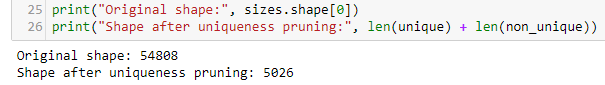
\includegraphics[width=\textwidth]{img/screen_shape.png}
\caption{Capture d'écran du nombre de lignes avant et après élagage\label{screen_shape}}
\end{figure}

Manuellement, nous avons alors défini des zones simples (rectangulaires) en tant que régions de décision de la plausibilité des dimensions des véhicules (Table \ref{regions_decision_manuelles_valeurs}). Ces zones ont été définies au jugé, afin d'encadrer le plus de points valides sans toutefois englober une zone de l'espace trop large. Une approche pour déterminer ces seuils peut être l'utilisation des records de taille enregistrés au cours de l'histoire.

\begin{table}
\centering
\begin{tabular}{llll}
cadre & validité & intervalle de longueur & intervalle de largeur \\
\hline
vert & non-malicieux & 3 à 6,5 mètres & 1,4 à 2,4 mètres \\
gris & malicieux & 3 à 4,1 mètres & 2,05 à 2,4 mètres \\
gris & malicieux & 5,25 à 6,5 mètres & 1,4 à 1,65 mètres \\
\end{tabular}
\caption{Dimensions des régions de décision arbitraires\label{regions_decision_manuelles_valeurs}}
\end{table}

Hors de la zone verte, et dans les deux cadres gris, nous avons alors généré aléatoirement 700 points définis comme malicieux. La Figure \ref{regions_decision_manuelles_plot} représente l'affichage de tous les points décrits plus tôt ainsi que des régions de décision. Ainsi faite, notre classification possède, sur le jeu d'entraînement, une précision de 97,83\%, et une précision de 97,31\%. Ces scores peuvent sembler suffisants, mais les régions de décisions montrées dans la Figure \ref{regions_decision_manuelles_plot} montrent qu'il y a des zones mortes (par exemple, pour une largeur supérieure à 2,1 mètres et une longueur supérieure à 5 mètres, dans lesquelles un attaquant pourrait positionner ses points malicieux. Ce modèle présente donc de l'\emph{underfitting}.

\begin{figure}
\centering
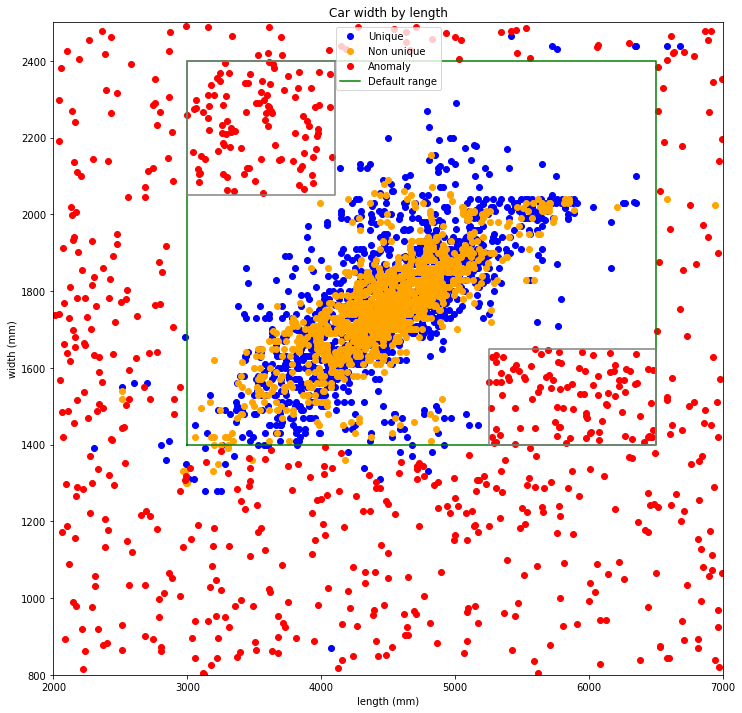
\includegraphics[width=\textwidth]{img/first_try.png}
\caption{Régions de décision manuelles pour des dimensions de voitures\label{regions_decision_manuelles_plot}}
\end{figure}

\section{Recherche des bases de données}

%TODO 

\section{Environnement de travail}

Dans cette partie, nous décrivons les outils utilisés et développés pour poursuivre notre étude. Ces éléments se retrouvent sur le dépôt git que nous avons utilisé pour sauvegarder notre code \cite{git}.

\subsection{Chargement des bases de données}

Afin de centraliser le chargement des bases de données explicitées plus tôt entre tous les scripts en ayant besoin, nous avons implémenté une fonction de chargement nommée \texttt{load\_detector} dans loader.py. Cette fonction instancie un object de la classe Detector, que nous décrirons dans la partie suivante. Elle procède de la façon suivante :

\begin{enumerate}
\item Pour chaque jeu de données au format CSV
\begin{enumerate}[{1.}1.]
\item Lire les colonnes contenant la longueur et la largeur
\item Renommer ces colonnes en "\texttt{length}" et "\texttt{width}"
\item Supprimer les lignes incomplètes
\item Si nécessaire, convertir les données en flottant et en millimètres
\item Ajouter une colonne contenant la classe correspondant au jeu de données considéré
\item Appliquer un premier filtre sur la longueur ou la largeur pour supprimer les points extrêmes isolés
\end{enumerate}
\item Fusionner toutes les matrices précédentes en une seule
\item Créer un nouvel objet \texttt{Detector} avec cette matrice en attribut
\item Supprimer les éventuels redondances
\item Ajouter une colonne "\texttt{odd}" à la matrice, initialisée à \texttt{False}
\item \textbf{Générer les données malicieuses}
\item Ajouter les données malicieuses à la base de données, en rajoutant la colonne "\texttt{odd}" initialisée à \texttt{True}
\item Remplacer les valeurs des classes (originnellement des chaînes de caractères comme \texttt{"car"} ou \texttt{"human"}) par des entiers
\item \textbf{Séparer la matrice en un jeu d'entraînement et un jeu de test}
\item Renvoyer l'objet `Detector` ainsi initialisé
\end{enumerate}

Dans le cas des bases de données décrites au paragraphe précédent, l'étape 1.6. permet de supprimer quelques points, par exemple une moto de longueur supérieure à 20 mètres, ou une voiture de 6 mètres de large. Bien que réelles, ces données sont trop isolées pour être considérés dans le reste de notre travail.

La DataFrame finale possède 4 colonnes, plus une pour l'index. Ces colonnes sont la classe du véhicule (entier), la longueur (flottant), la largeur (flottant), et le caractère malicieux (booléen).

\paragraph{Génération des données malicieuses} \textit{Toutes les données que nous avons recueillies proviennent de base de données légitimes. Afin d'obtenir des données malicieuses afin d'entraîner nos classeurs, nous avons procédé à une génération manuelle de ces dernières. Nous nous sommes concentré sur une génération uniforme, ce qui peut correspondre à une attaque d'aveuglement des capteurs.} ~\par Pour un nombre de points à générer donné, le programme génère des points uniformément dans la zone rectangulaire définie par les minimums et maximums de longueur et de largeur de la base de données initiales. À chacun de ces points est associé, uniformément, une classe aléatoire parmi les classes présentes dans la base de données. La génération utilise un \emph{seed} entier entre 0 et $2^{32}-1$, ré-utilisable ultérieurement pour générer le même jeu de données.

\paragraph{Séparation de la matrice} La matrice est pour l'instant stockée en tant qu'attribut de l'objet \texttt{Detector}. Avec le \emph{seed} généré précédemment, elle est tout d'abord mélangée pour éviter d'avoir toutes les données triées. Puis, elle est coupée en deux moitiés :
\begin{itemize}
\item le jeu d'entraînement
\item le jeu de test
\end{itemize}
La première moitié servira à entraîner nos classeurs, tandis que la seconde nous permettra de confronter ces classeurs à des données réelles, sélectionner les paramètres et définir le meilleur classeur.

Enfin, on procède à la division de chacune de ces matrices en deux matrices, une pour les \emph{features} et une pour le label de sortie (le caractère malicieux). Au final, chacune de ces DataFrames (\texttt{x\_train}, \texttt{y\_train}, \texttt{x\_test} et \texttt{y\_test}) est stockée dans l'objet \texttt{Detector}. La figure \ref{xtrain} montre les 10 premières lignes de \texttt{x\_train}\label{features_matrix}.

\begin{figure}
\centering
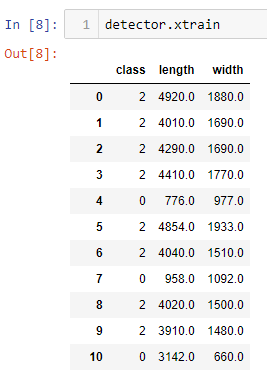
\includegraphics[scale=.8]{img/xtrain.png}
\caption{Premières lignes de la matrice de \emph{features} du jeu d'entraînement\label{xtrain}}
\end{figure}

\subsection{Classe \texttt{Detector}}

Comme expliqué précédemment, cette classe stocke les jeux de données utilisés pour l'entraînement et la prédiction. Elle va aussi permettre de centraliser les tests de classeurs, et l'affichage des données. Ses méthodes (Table \ref{methodes_detector}) sont donc une sorte d'API pour la réalisation de la fonction de prédiction finale, objectif du projet.

\begin{table}
\centering
\begin{tabular}{p{2.3cm} p{3.1cm} p{4.6cm}}

\multirow{6}{*}{Pre-processing}& \multirow{2}{*}{\texttt{clean}} & Étapes 4 et 5 du chargement des bases de données \\
& \multirow{2}{*}{\texttt{append\_odd\_points}} & Étape 7 du chargement des bases de données \\
& \multirow{2}{*}{\texttt{format}} & Étapes 8 et 9 du chargement des bases de données \\
\hline
& \multirow{3}{*}{\texttt{classify}} & Entraîne un classeur et renvoie la matrice de confusion sur le jeu de test\\
Interface \par \texttt{sklearn} & \multirow{2}{*}{\texttt{tune\_parameters}} & Trouve le meilleur jeu de paramètres pour un classeur \\
& \multirow{2}{*}{\texttt{predict}} & Fonction finale de prédiction online \\
\hline
\multirow{4}{*}{Affichage}& \multirow{2}{*}{\texttt{plot}} & Affiche la matrice de données complètes\\
& \texttt{plot\_decision\_}\par\texttt{boudaries} & Affiche les régions de décisions d'un classeur\\

\end{tabular}
\caption{Méthodes de la classe \texttt{Detector}\label{methodes_detector}}
\end{table}

\section{Méthode d'évaluation}


\subsection{Matrice de confusion}
Une technique pour évaluer la performance d'un algorithme de classification est d'utiliser une matrice de confusion. Il s'agit d'un résumé des résultats de prédiction sur un problème de classification, qui donne un aperçu du degré de confusion de notre modèle. 

\subsubsection{Terminologie}
Pour définir de manière formelle une matrice de confusion, il convient d'introduire les termes suivants : 
\begin{itemize}
\item TP (Vrai Positif): item correctement détecté positif 
\item FP (Faux Positif): item déclaré positif, là où il est en réalité négatif
\item FN (Faux négatif): item déclaré négatif alors qu'il était en réalité positif
\item TN (Vrai négatif): item correctement détecté comme négatif
\end{itemize}
\medskip
Ces derniers permettent de définir la classification, correcte ou non, des objets données en entrée de notre fonction. Nous pouvons dès lors construire la matrice suivante : 

\begin{tabular}{ l | l | c | c | c c}
\multicolumn{2}{c}{} & \multicolumn{2}{c}{Classe réelle} & \\
\cline{3-4}
\multicolumn{2}{c|}{} & Positif & Négatif \\
\cline{2-4}
\multirow{2}{*}{Classe prédite} & Positif & $TP$ & $FP$ & $PPV$ & $FDR$ \\
\cline{2-4}
& Négatif & $FN$ & $TN$ & $FOR$ & $NPV$ \\
\cline{2-4}
\multicolumn{1}{r}{} & \multicolumn{1}{l}{} & \multicolumn{1}{c}{$TPR$} & \multicolumn{1}{c}{$FPR$} \\
\multicolumn{1}{l}{} & \multicolumn{1}{l}{} & \multicolumn{1}{c}{$FNR$} & \multicolumn{1}{c}{$TNR$} \\
\end{tabular}

~\par
Les colonnes représentent le nombre d'occurrences d'une classe de référence (ie des observations issues de notre base de données). Les lignes quant à elles le nombre d'occurrences d'une classe estimés par notre modèle de classification. 
~\par
\medskip
Pour illustrer cette terminologie, nous introduisons la matrice de confusion suivante, obtenues en appliquant l'algorithme RandomForest sur notre base de données:

$$\begin{bmatrix}
2801 & 19 \\ 
36 & 467 \\
\end{bmatrix}$$

Ainsi, parmi les 2837 observations positives, 2801 seront estimés comme tels et 36 comme étant négatives. De même, sur les 2820 observations que notre modèle a estimé comme positives, 19 sont en réalité négatives. Le même raisonnement s'applique pour les observations négatives. 


Pour la suite, et pour comprendre cette matrice, il convient d'introduire les résultats suivants:

\begin{itemize}\setlength{\itemsep}{1.5mm}
\item ratio de vrai positif: $TPR=\dfrac{TP}{TP+FN}=0.987$  (true positive rate)

~\par

Ce ratio montre la capacité de notre modèle à détecter tous les valeurs positives. Ici, cette détection est très efficace. Néanmoins, il est important de noter que nous pouvons facilement avoir un très bon TPR en prédisant systématiquement "positif". Cette valeur doit donc s'interpréter avec celle du TNR. 

\item ratio de vrai négatif: $TNR=\dfrac{TN}{TN+FP} = 0.959$ (True negative rate)

~\par

Aussi appelé sensibilité. Mesure la capacité de notre modèle à détecter les valeurs négatives. De la même manière que pour le TPR, on peut facilement avoir un très bon TNR en prédisant systématiquement négatif. Ici, la valeur importante combinée à celle du TPR renforce la performance du modèle.

\item ratio de faux positif: $FPR=\dfrac{FP}{TP+TN}=0.04$ (False positive rate)

~\par

Ce ratio décrit en quelque sorte la probabilité de fausse alarme. 

\item ratio de faux négatif: $FNR=\dfrac{FN}{TP+FN}=0.01 $ (False negative rate)

~\par

Décrit en quelque sorte le ratio de mauvaise classification des items positifs. Un taux égal à 1 signifierait que 100\% des items positifs ont été déclaré négatifs. On remarque que notre modèle classifie avec efficacité les items positifs.

\item valeur prédictive positive: $PPV=\dfrac{TP}{TP+FP}=0.993$  (positive predicted value)

~\par

Une PPV importante signifie qu'un item marqué positif est réellement positif (il y a un faible nombre de faux positifs). 

\item valeur prédictive négative: $NPV=\dfrac{TN}{TN+FN}=0.928$ (negative predicted value)

~\par

A l'inverse du PPV, un NPV important signifie qu'un item marqué négatif est réellement négatif (il y a un faible nombre de faux négatif).


\item taux de fausses découvertes: $FDR=\dfrac{FP}{TP+FP}=0.001$   (False discovery rate)

~\par

Il s'agit du complémentaire de la précision. Un FDR important signifie l'incapacité de notre modèle à détecter les items positifs. 

\item taux de fausses omissions: $FOR=\dfrac{FN}{TN+FN}=0.072$ (False omission rate)

~\par

Il s'agit du complémentaire du NPV. Un FOR important indique l'incapacité de notre modèle à détecter les items négatifs. 

\end{itemize}

~\par

Ce mode de représentation permet non seulement de mettre en évidence les erreurs qui sont faites par notre classeur, mais surtout des types d'erreurs (mauvaise détection d'une classe ou surestimation du des items positifs par exemple) qui sont commises. En effet, l'utilisation de la seule “accuracy” peut être trompeuse dans la mesure où le nombre d'observations dans chaque classe est inégale. \\
\medskip
Pour illustrer ce phénomène, prenons un exemple précis. Considérons l'algorithme SVM (support vector Machine) avec les paramètres suivants:
\medbreak

\begin{center}
\noindent
\fbox{\begin{minipage}[t]{.9\textwidth}\begin{small}
C=0.1, cache--size=200, class--weight=None, coef0=0.0, decision--function--shape='ovr', degree=3, gamma='auto', kernel='linear', max--iter=-1, probability=False, randomState=None, shrinking=True,  tol=1e-05, verbose=False
\end{small}\end{minipage}}
\end{center}
\medbreak
Cet algorithme renvoie avec notre base de donnée, la matrice de confusion suivante: 

$$\begin{bmatrix}
2771 & 74 \\ 
239 & 239 \\
\end{bmatrix}$$

\bigskip
L'accuracy est égale à:

\begin{equation}
 accuracy=\dfrac{TP+TN}{\text{Total items}}= 0.91
\end{equation}

\medskip

Nous remarquons que 313 items ont mal été classifiés. Dans le cadre d'une classification d'obstacles, cela est loin d'être satisfaisante alors que le score d'accuracy est, lui, relativement important. Il y a en effet dans ce dernier aucune pondération. Si une classe contenant un nombre de paramètres important est bien classifiée, elle peut "masquer" les mauvais résultats obtenus pour d'autres classes plus petites.

\subsubsection{Score F1}
Comme nous l'avons vu, le taux d'accuracy reste trop général pour correctement caractériser la performance d'une classification. En effet, il n'est pas pondéré selon le nombre d'élément de chaque classe ce qui peut induire des erreurs d'appréciation. Nous allons donc utiliser une autre métrique: le score F1. Pour ce faire, introduisons deux termes:

\begin{description}
\item[La précision :] la précision est le ratio d'observations positives correctement prédites sur le total des observations positives prédites. Une précision importante signifie qu'un item marqué positif l'est réellement. On a donc : \begin{equation}
\text{Precision} = \dfrac{TP}{TP+FP}
\end{equation}
\item[Le taux de rappel :] le taux de rappel montre la capacité de notre modèle à détecter tous les valeurs positives. On a: \begin{equation}
\text{Recall} = \dfrac{TP}{TP+FN}
\end{equation}
\end{description}

Il est souvent intéressant de comparer deux versions d'un classeur pour déterminer lequel est le plus performant. Une idée intuitive serait de faire la moyenne de la précision et du taux de rappel. Pourtant cette idée est loin d'être la meilleure. Considérons par exemple deux cas:
\begin{itemize}

\item Cas 1: Taux de rappel élevé, faible précision: Cela signifie que la plupart des exemples positifs sont correctement reconnus (FN faible) mais il y a beaucoup de faux positifs.

\item Cas 2: Faible taux de rappel, haute précision: Cela montre que nous manquons beaucoup d'items positifs (FN élevé) mais ceux que nous pronostiquons positifs le sont en effet (FP faible)
\end{itemize}

\medskip
Ainsi, dans le cas d'une précision très mauvaise et d'un taux de rappel très élevé (ou inversement), nous pouvons rapidement arriver à une mauvaise estimation de la performance de notre algorithme. C'est pour cette raison que nous introduisons une nouvelle métrique: \textbf{le score F1}. Elle est définie comme étant la moyenne harmonique de la précision et du taux de rappel. On a donc:
\begin{equation}
	\text{f1-score} = \dfrac{2\times(\text{Recall} \times \text{Precision})}{(\text{Recall} + \text{Precision})} = 2\times\dfrac{PPV \times TPR}{PPV + TPR}
\end{equation}

Dans notre cas, nous cherchons à minimiser le nombre de faux positifs et de faux négatifs. L'utilisation du score F1 nous permet de les prendre tous deux en compte.

\chapter{Paramétrage et résultats}

\section{Recherche des paramètres optimaux}

À cette étape du projet, nous avions utilisés différents classeurs mais laissé les paramètres de ces derniers aux valeurs par défaut. Les résultats étaient assez mauvais pour SVM, le perceptron multi-couches et AdaBoost. Seule la Random Forest semblait se comporter correctement. Nous nous sommes donc penché sur l'optimisation des paramètres des trois premiers classeurs cités.

Une majeure partie de notre temps a été investie dans la recherche des jeux de paramètres optimaux pour chacun des classeurs sélectionnés. Nous avons procédé en deux temps. Premièrement, nous avons implémenté un script testant des intervalles de paramètres et renvoyant les meilleurs combinaisons. Puis, nous avons utilisé ce script pour des intervalles de valeurs de paramètres que nous avons jugé pertinents.

\subsection{Recherche exhaustive et validation croisée}

Notre algorithme de recherche des paramètres est basé sur une fonction de scikit-learn, dans le module de sélection de modèle : \texttt{GridSearchCV}. Cette fonction est utilisée dans la méthode \texttt{tune\_parameters} du \texttt{Detector}. Cette fonction effectue une recherche exhaustive d'un jeu de paramètres optimal pour un classeur donné à partir d'un dictionnaire Python\footnote{Conteneur pouvant être indexé par n'importe quel objet dont Python peut produire un \emph{hash}. Le fonctionnement est similaire à une table de hachage en C ou une Map en Java.}, dont les clés (index) sont les paramètres à faire varier et les valeurs les listes des valeurs prises par ces paramètres.

Cette fonction utilise de plus la technique de validation croisée. En quelques mots, cette technique consiste en la division des données d'entraînement en $C$ sous-échantillons. De façon cyclique, 1 sous-échantillon servira à la validation du modèle, tandis que les $C-1$ autres permettront l'entraînement du modèle. On répète la technique de validation croisée $C$ fois, afin que chaque sous-échantillon soit utilisé pour la validation une fois. La performance du modèle est ensuite évaluée en moyennant les scores de chaque itération. Cette méthode permet de prédire l'efficacité d'un classeur en évitant tout phénomène d'\emph{overfitting} sans avoir à disposer d'un jeu de test indépendant.

La fonction d'évaluation du score utilisée par \texttt{GridSearchCV} est par ailleurs paramétrable. Dans le cadre de notre projet, nous nous intéressons au \emph{f1-score} pour évaluer un classeur, et nous souhaitions aussi extraire les tendances de l'évolution du score en fonction des différents paramètres testés. Nous pourrons alors interpréter l'impact des différents paramètres, et expliquer leur rôle. Nous avons donc implémenté notre propre fonction d'évaluation, prenant en paramètre le classeur à évaluer (Section \ref{classifiers}) et les matrices de \emph{features} et de \emph{labels} (Section \ref{features_matrix}) à utiliser pour cela. Cette fonction effectue les opérations suivantes :

\begin{enumerate}
\item Classification des éléments du jeu de test (ici, le sous-échantillon mentionné dans la validation croisée). Production d'une matrice de \emph{labels}, contenant les classes résultant de la classification.
\item Calcul de la matrice de confusion entre la prédiction et la matrice donnée en consigne. Parmi les données qui viennent d'être classé, on compte le nombre de vrais positifs, de vrais négatifs, de faux positifs et de faux négatifs.
\item Sauvegarde des paramètres et du score
\item Retour du \emph{f1-score}
\end{enumerate}

L'étape 3 consiste en l'écriture dans un fichier d'une ligne contenant la description détaillée des paramètres du classeur ainsi que les résultats des scores. La fonction de recherche exhaustive étant fortement parallèle, chaque processus écrit dans son propre fichier. Une fois tous les tests effectués, ces fichiers sont concaténés en un grand fichier. Cette méthode d'enregistrement continu permet en outre de sauvegarder les résultats des tests successifs des itérations de la validation croisée au fur et à mesure de l'exécution du programme, ce qui se révèlera important lors d'interruptions prématurées de cette exécution.

En effet, ce fut l'un de nos plus importants problèmes lors de ce projet. Pour le Multi-layered Perceptron, il y avait beaucoup de paramètres en jeu, et la complexité combinatoire mélangée avec le temps de convergence des réseaux neuronaux ont rendu le temps d'exécution du script interminable. Notre plus long essai eut lieu sur le serveur InfRes \href{http://lame10.enst.fr}{lame10} doté pourtant de 80 CPUs, sur une durée de plus de 18 heures ; l'intégralité des tests n'aura pu être effectuée, nous avons dû manuellement interrompre l'exécution.

Enfin, du grand fichier généré contenant l'historique de tous les tests passés sont ensuite extraites les tables de score CSV qui seront présentées dans les paragraphes suivant. Ces dernières sont disponibles en ligne\footnote{\url{https://perso.telecom-paristech.fr/ychalier/anomaly/params/}}. Pour chaque phase de test, le script génère :
\begin{itemize}
\item Un fichier de scores (TPR, FPR, TNR, FNR, PPV, \emph{f1-score}, temps de prédiction)
\item Pour chaque classe différente de classeur, un fichier contenant tous les jeux de paramètres
\end{itemize}
Ces tables sont, à la manière des tables en SQL, liées par une clé primaire externe qui est l'identifiant (unique) de la combinaison de paramètres.

%TODO : perspective : bloquer les paramètres reconnus comme meilleurs et faire varier ceux qui semblent useless, peut-être qu'une tendance va émerger

\subsection{Multi-layered perceptron}

À l'aide d'un autre petit script Python, nous avons pu afficher les données récoltées dans les CSV mentionnés plus tôt. Les Figures \ref{mlp_activation} et \ref{mlp_solver} sont le résultat du test pour les paramètres du MLP. La Table \ref{params_mlp} regroupe les différents paramètres testés, à savoir :
\begin{description}
\item[learning rate] Taux de modification des poids à chaque mise à jour (i.e. à chaque rétropropagation)
\item[alpha] Pénalité de régularisation (en utilisant la norme $l_2$)
\item[activation] Fonction d'activation du réseau neuronal
\item[solver] Algorithme de descente du gradient
\item[hidden layers size] Nombre et taille des couches cachées du réseau
\end{description}

\begin{table}
\centering
\begin{tabular}{l l}
paramètre & ensemble des valeurs testées \\
\hline
\texttt{learning\_rate} & \texttt{'constant'}, \texttt{'invscaling'} et \texttt{'adaptive'}\\
\texttt{alpha} & $\{10^{-k} \>\> | \>\> k \in [\![4, 7]\!] \}$ \\
\texttt{activation} & \texttt{'identity'}, \texttt{'logistic'}, \texttt{'tanh'} et \texttt{'relu'} \\
\texttt{solver} &\texttt{'lbfgs'}, \texttt{'sgd'} et \texttt{'adam'}\\
\texttt{hidden\_layer\_sizes} & 0 à 5 \emph{layers}, de taille variant de 1 à 49\\
\end{tabular}
\caption{Liste des paramètres testés pour le multi-layered perceptron\label{params_mlp}}
\end{table}

L'exploitation des résultats est rendue très difficile par le manque de consistance des scores. Cependant, nous avons pu remarqués que des paramètres comme la régularisation (\texttt{alpha}) ou la taille et nombre de \emph{layers} n'avaient que peu d'influence sur les résultats. Par contre, deux éléments semblent ce dégager : \begin{itemize}
\item la tangente hyperbolique comme fonction d'activation (Figure \ref{mlp_activation})
\item \emph{lbfgs} comme méthode du gradient (la documentation de sklearn prédit cette préférence lorsqu'il y a peu de données à exploiter) (Figure \ref{mlp_solver})
\end{itemize}
Enfin, la Table \ref{best_params_mlp} donne les résultats donnés par la recherche exhaustive et validation croisée (pour un \emph{f1-score} moyen maximal de 0.937, ce qui est très prometteur).

\begin{table}
\centering
\begin{tabular}{ll}
paramètre & valeur \\
\hline
\texttt{learning\_rate} & \texttt{'constant'} \\
\texttt{alpha} & \texttt{$10^{-6}$} \\
\texttt{activation} & \texttt{'tanh'} \\
\texttt{solver} & \texttt{'lbfgs'} \\
\texttt{hidden\_layer\_sizes} & \texttt{[28, 28, 28]}\\
\end{tabular}
\caption{Paramètres optimaux pour MLP\label{best_params_mlp}}
\end{table}

\paragraph{Remarque} Sur les Figures \ref{mlp_activation} et \ref{mlp_solver}, nous pouvons observer une "barre" en (0,0). Ces points correspondent aux tests avec 0 couches cachées (qui sont, par convention, de taille nulle). Les résultats ne sont donc pas étalés comme pour les autres tailles.

\begin{figure}
\centering
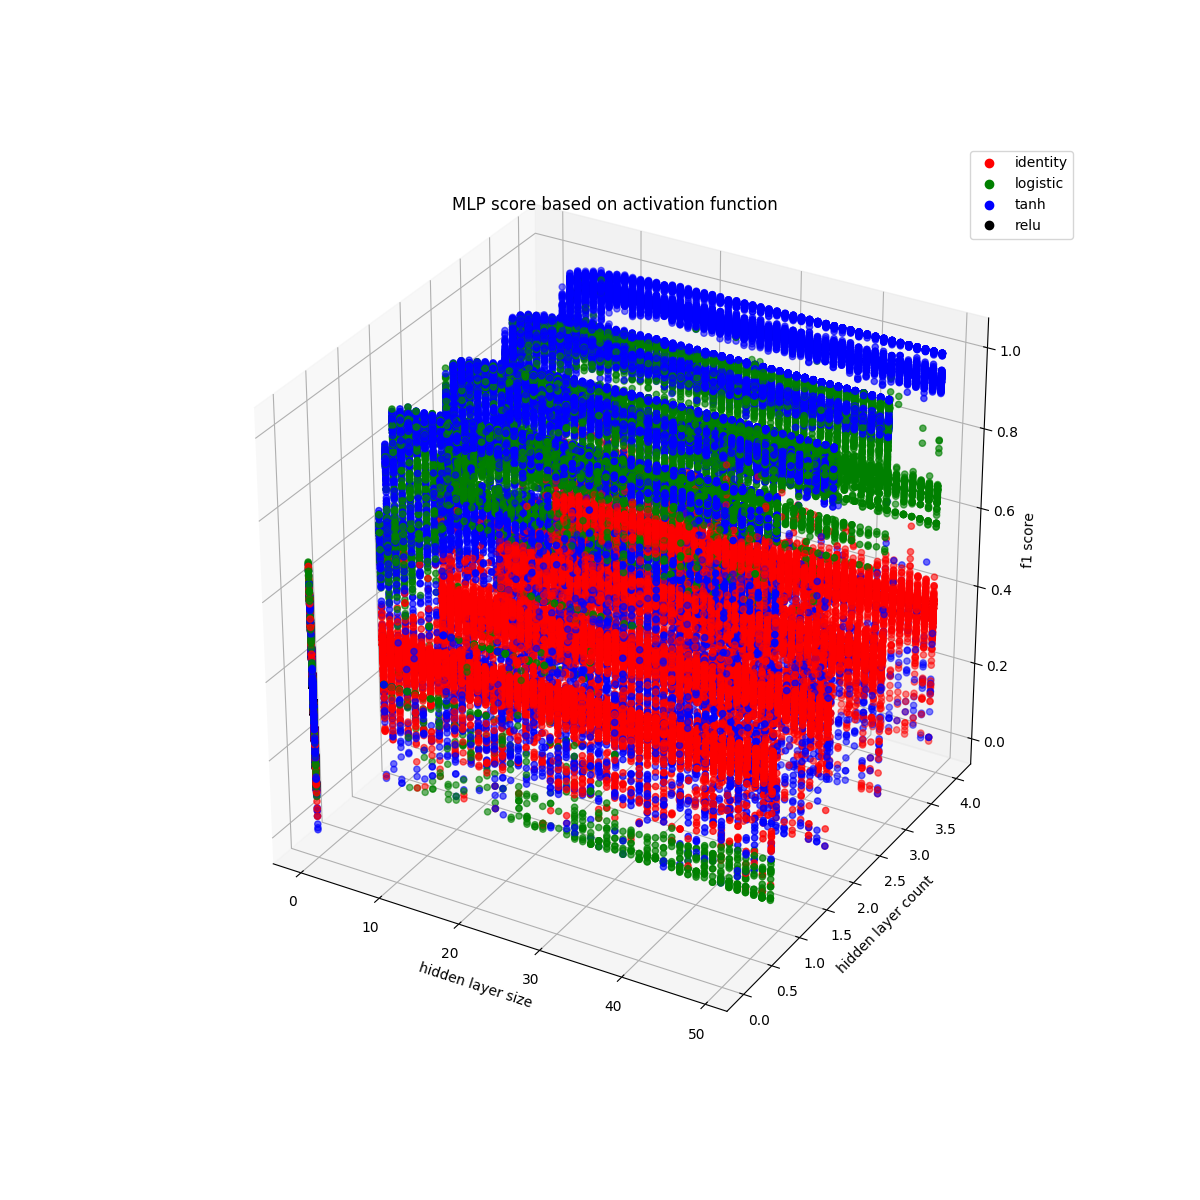
\includegraphics[width=\textwidth]{img/mlp_activation.png}
\caption{Évolution du \emph{f1-score} pour MLP selon la fonction d'activation\label{mlp_activation}}
\end{figure}

\begin{figure}
\centering
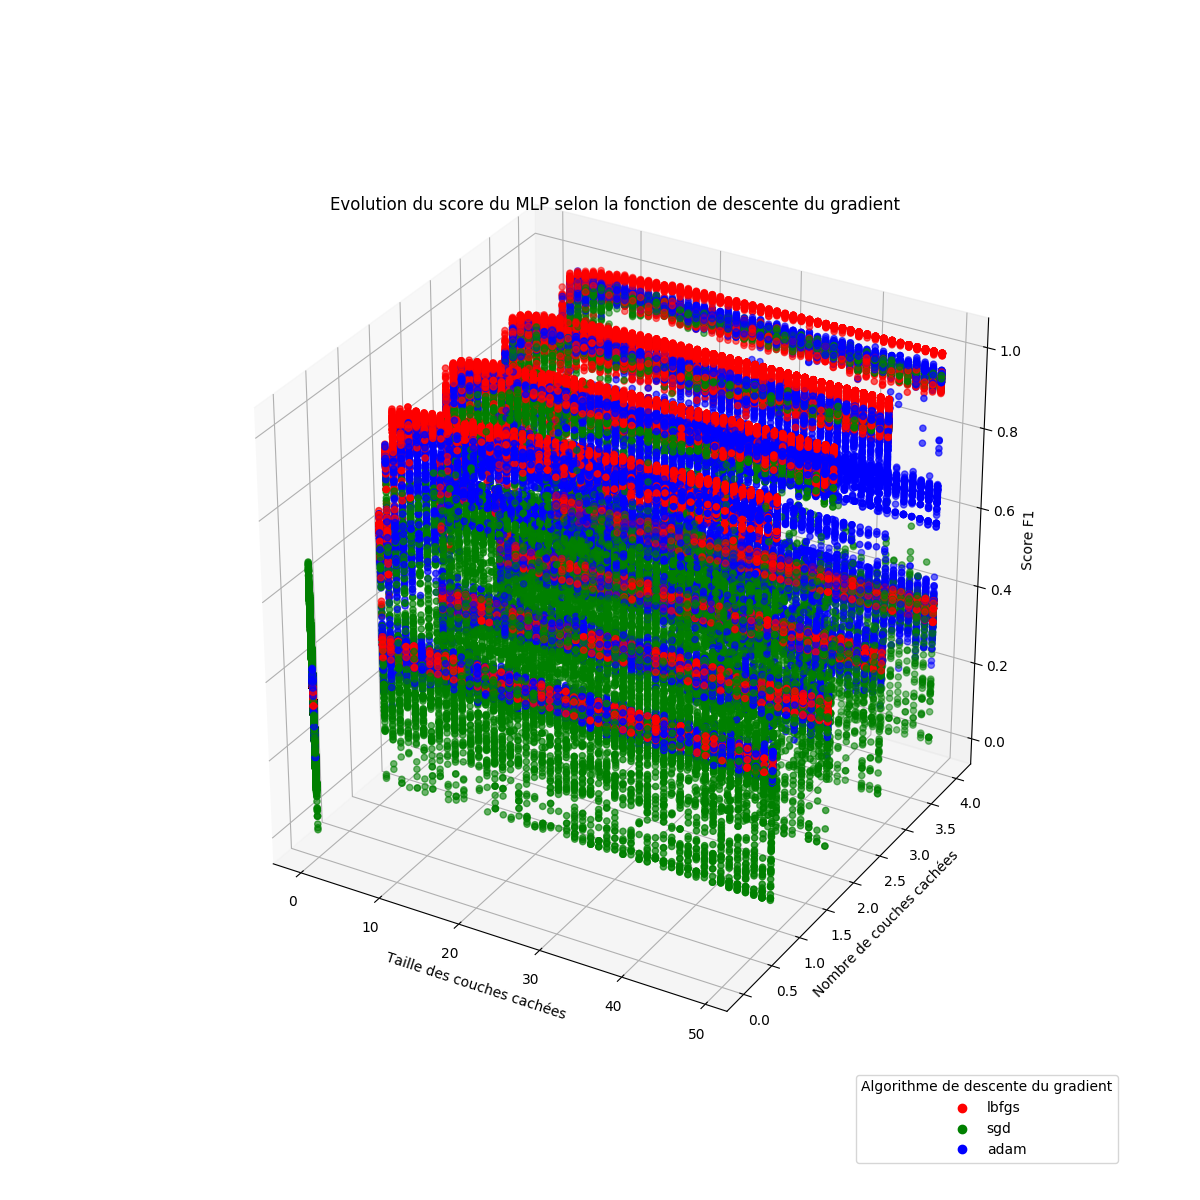
\includegraphics[width=\textwidth]{img/mlp_solver.png}
\caption{Évolution du \emph{f1-score} pour MLP selon l'algorithme de descente du gradient\label{mlp_solver}}
\end{figure}

\subsection{AdaBoost}

Comme pour MLP, la Table \ref{params_ada} liste les paramètres testés et la Figure \ref{adaboost_depth} montre l'évolution du score en fonction de ces paramètres.

\begin{table}
\centering
\begin{tabular}{ll}
paramètre & ensemble des valeurs testées \\
\hline
\texttt{n\_estimators} & $[\![1, 99]\!]$ \\
\texttt{learning\_rate} & $\{k/10 \>\> | \>\> k \in [\![1, 9]\!] \}$ \\
\texttt{base\_estimator} & Arbres de décision de profondeur maximale dans $[\![2, 9]\!]$\\
\end{tabular}
\caption{Liste des paramètres testés pour AdaBoost\label{params_ada}}
\end{table}

Ici, il y a peu d'interprétations possibles : les paramètres influent peu sur la performance du classeur. Dès lors que les arbres sont suffisamment profonds, qu'il y a assez d'estimateurs agrégés et que le taux d'apprentissage est correct (supérieur à 0.1), les résultats sont vite optimaux. La fonction de recherche exhaustive nous a renvoyé la combinaison de paramètres présentée dans la Table \ref{best_params_ada} (pour un \emph{f1-score} moyen maximal de 0,947, proche de celui du MLP, tout aussi prometteur).

\begin{table}
\centering
\begin{tabular}{ll}
paramètre & valeur \\
\hline
\texttt{n\_estimators} & 46 \\
\texttt{learning\_rate} & 0,3 \\
\texttt{base\_estimator} & Arbres de décision de profondeur maximale 3\\
\end{tabular}
\caption{Paramètres optimaux pour AdaBoost\label{best_params_ada}}
\end{table}

\begin{figure}
\centering
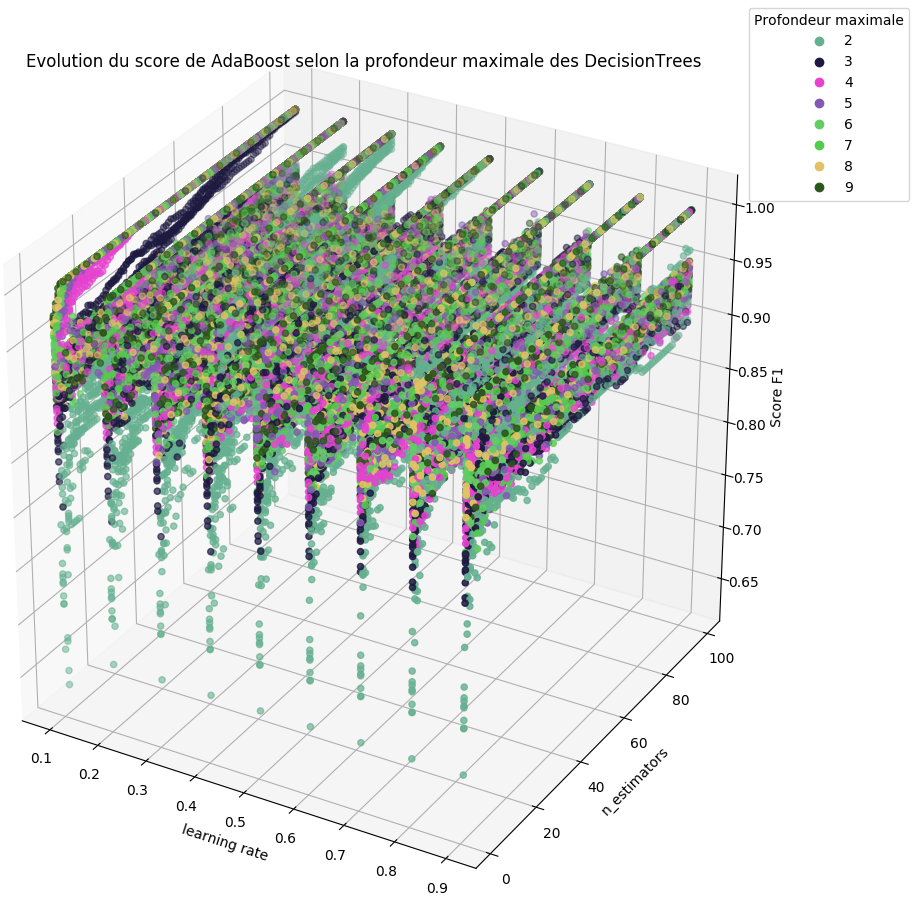
\includegraphics[width=\textwidth]{img/adaboost_depth.png}
\caption{Évolution du \emph{f1-score} pour AdaBoost selon la profondeur maximale de l'arbre de décision\label{adaboost_depth}}
\end{figure}

\subsection{SVM}

L'algorithme du SVM est initialement défini pour la discrimination d'une variable qualitative binaire; c'est à dire des variables contenant deux éléments non ordonnables (eg la variable sexe contient les éléments masculin et féminin. Il est à ce titre particulièrement indiqué dans le cas de problèmes linéairement séparables. On cherche donc un hyperplan capable de séparer l'espace vectoriel en deux. Or, nous sommes en présence d'un problème à trois classes. Nous ne pouvons donc pas trouver un unique hyperplan qui séparerait notre espace. Nous allons donc devoir adapter la méthode générale. Plusieurs adaptations existent. Parmi ces dernières, nous avons considéré les deux suivantes :

\begin{description}
\item["One-Versus-the-Rest"] La plus simple et la plus ancienne des méthodes d'otpimisation indirectes. Il s'agit d'une extension au cas multiclasses proposée par Vapnik \cite{Vapnik}. Elle consiste à construire $p$ estimateurs binaires (à vecteurs de supports) pour classifier $p$ classes. S'il s'agit d'une extension facile à mettre en place, cette méthode risque d'introduire artificiellement un déséquilibre des classes dans la construction des modèles individuels. Dans notre cas, nous avons 70847 points représentants des voitures contre 202 représentants des motos. Aussi, la méthode SVM obtiendra des moins bons résutlats pour séparer ces deux classes.

\begin{figure}
\centering
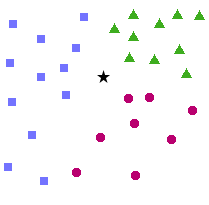
\includegraphics[scale=0.6]{img/svm.png}

\includegraphics[scale=0.6]{img/svm_OneVsAll.png}
\caption{Problème multi-classe et séparation "One-Versus-the-Rest"}
\end{figure}

\item[Méthode directe de Crammer et Singer \cite{Crammer}] À l'encontre des schémas de décomposition indirect (comme la méthode "OVR"), cette approche cons\-iste à séparer les classes en résolvant un unique problème d'optimisation. Ainsi, cela revient à résoudre un problème d'optimisation à $n(p-1)$ contraintes (où $p$ est le nombre de classe et $n$ le nombre d'observations).
\end{description}
Comme pour les méthodes précédentes, la Table \ref{params_svm} liste les paramètres testés.

\begin{table}
\centering
\begin{tabular}{ll}
paramètre & ensemble des valeurs testées \\
\hline
\texttt{multi\_class} & \texttt{'ovr'}, \texttt{'crammer\_singer'} \\
\texttt{C} & $\{10^k \>\> | \>\> k \in [\![-2, 3]\!] \}$ \\
\texttt{tol} & $\{10^{-k} \>\> | \>\> k \in [\![3, 6]\!] \}$ \\
\end{tabular}
\caption{Liste des paramètres testés pour SVM\label{params_svm}}
\end{table}

\noindent Pour implémenter cette méthode, nous avons utilisé la fonction linearSVC de la bibiliothèque SKlearn. Cette fonction, similaire à SVC avec le paramètre kernel='linear', est implémenté différement et propose plus de flexibilité dans le choix des pénalités et des fonctions de perte. Elle s'adapte donc mieux à un grand nombre d'échantillons. Pour tous les essais, \texttt{LinearSVC} a eu pour paramètres \begin{center}
\texttt{penalty='l1'} et \texttt{dual=False}
\end{center}
En effet, comme nous avons trois classes pour deux caractéristiques de sélection, il est plus performant de résoudre le problème primal (par défaut, le dual est sélectionné). De plus, \texttt{GridsearchCV} ne permet pas la combinaison de la résolution du problème primal et de la norme 2 comme fonction de pénalisation. %TODO : finir phrase

Nous avons obtenu le meilleur résultat avec la combinaison des paramètres présentée dans la Table \ref{best_params_svm}.

\begin{table}
\centering
\begin{tabular}{ll}
paramètre & valeur \\
\hline
\texttt{multi\_class} & crammer\_singer \\
\texttt{C} & 100 \\
\texttt{tol} & 0.00001\\
\end{tabular}
\caption{Paramètres optimaux pour SVM\label{best_params_svm}}
\end{table}

Pour ces paramètres, nous obtenons la matrice de confusion suivante :
$$\begin{bmatrix}
2836 & 1 \\ 
400 & 86 \\
\end{bmatrix}$$
Il faut tout de même noter que ces résultats sont sujets à des fortes variations.

\section{Étude comparative des performances}

\section{Utilisation de la prédiction en-ligne}

L'objectif final de ce projet est la mise à disposition d'une fonction de prédiction autonome permettant de classer des données relevées par un ensemble de capteurs en malicieux / non-malicieux.

Cette fonction est déjà implémentée dans le code, il s'agit de la méthode \texttt{predict} de la classe \texttt{Detector}. Le processus pour initialiser cette fonction est le suivant :
\begin{enumerate}
\item Créer un objet \texttt{Detector} en chargeant les bases de données récoltées
\item Entraîner un classeur, dont les paramètres sont ceux résultant de l'optimisation effectuée précédemment, avec ces données
\item Attribuer ce classeur en tant que classeur de prédiction pour le \texttt{Detector}
\item Sauvegarder la méthode \texttt{predict}
\end{enumerate}
La dernière étape de ce processus consiste en la sérialisation de la méthode, à l'aide du module Pickle. Ce module permet d'écrire octet par octet la fonction telle qu'elle est représentée dans la RAM de Python, pour pouvoir la recharger plus tard et l'appeler telle une fonction normale. En effet, la méthode contient une référence au classeur sélectionné (en attribut de l'objet référent). Par un effet de fermeture\footnote{La fonction utilise des variables indépendantes (utilisées localement mais définies dans la portée englobante). Autrement dit, ces fonctions se souviennent de l'environnement dans lequel elles ont été créées.}, cette valeur sera aussi enregistrée lors de la sérialisation de la méthode. La fonction possède donc tous les éléments pour effectuer les prédictions. Elle est stockée dans un fichier \emph{anomaly\_classifier.clf}. Son utilisation peut alors être résumée à l'aide de la fonction suivante :
\begin{verbatim}
def classify(class_, length, width):
    import pickle
    
    # Ouverture du fichier contenant la fonction
    # en mode de lecture binaire
    file = open('anomaly_classifier.clf', 'rb')
    
    # Chargement du contenu du fichier dans la RAM,
    # et stockage de la référence de la fonction
    # dans la variable fun
    fun = pickle.load(file)
    file.close()
    
    # Classification
    if fun(class_, length, width):
        return "malicious"
    else:
        return "non-malicous"
\end{verbatim}
Cette fonction est autonome, elle n'a plus besoin de l'objet \texttt{Detector} pour fonctionner. De plus, elle est portable, puisqu'elle ne nécessite qu'un fichier contenant la méthode citée précédemment, fichier pesant environ 400Ko, ce qui est bien inférieur à la taille des bases de données nécessaires pour entraîner le classeur (14 Mo).

\chapter{Conclusions}

\begin{figure}
\centering
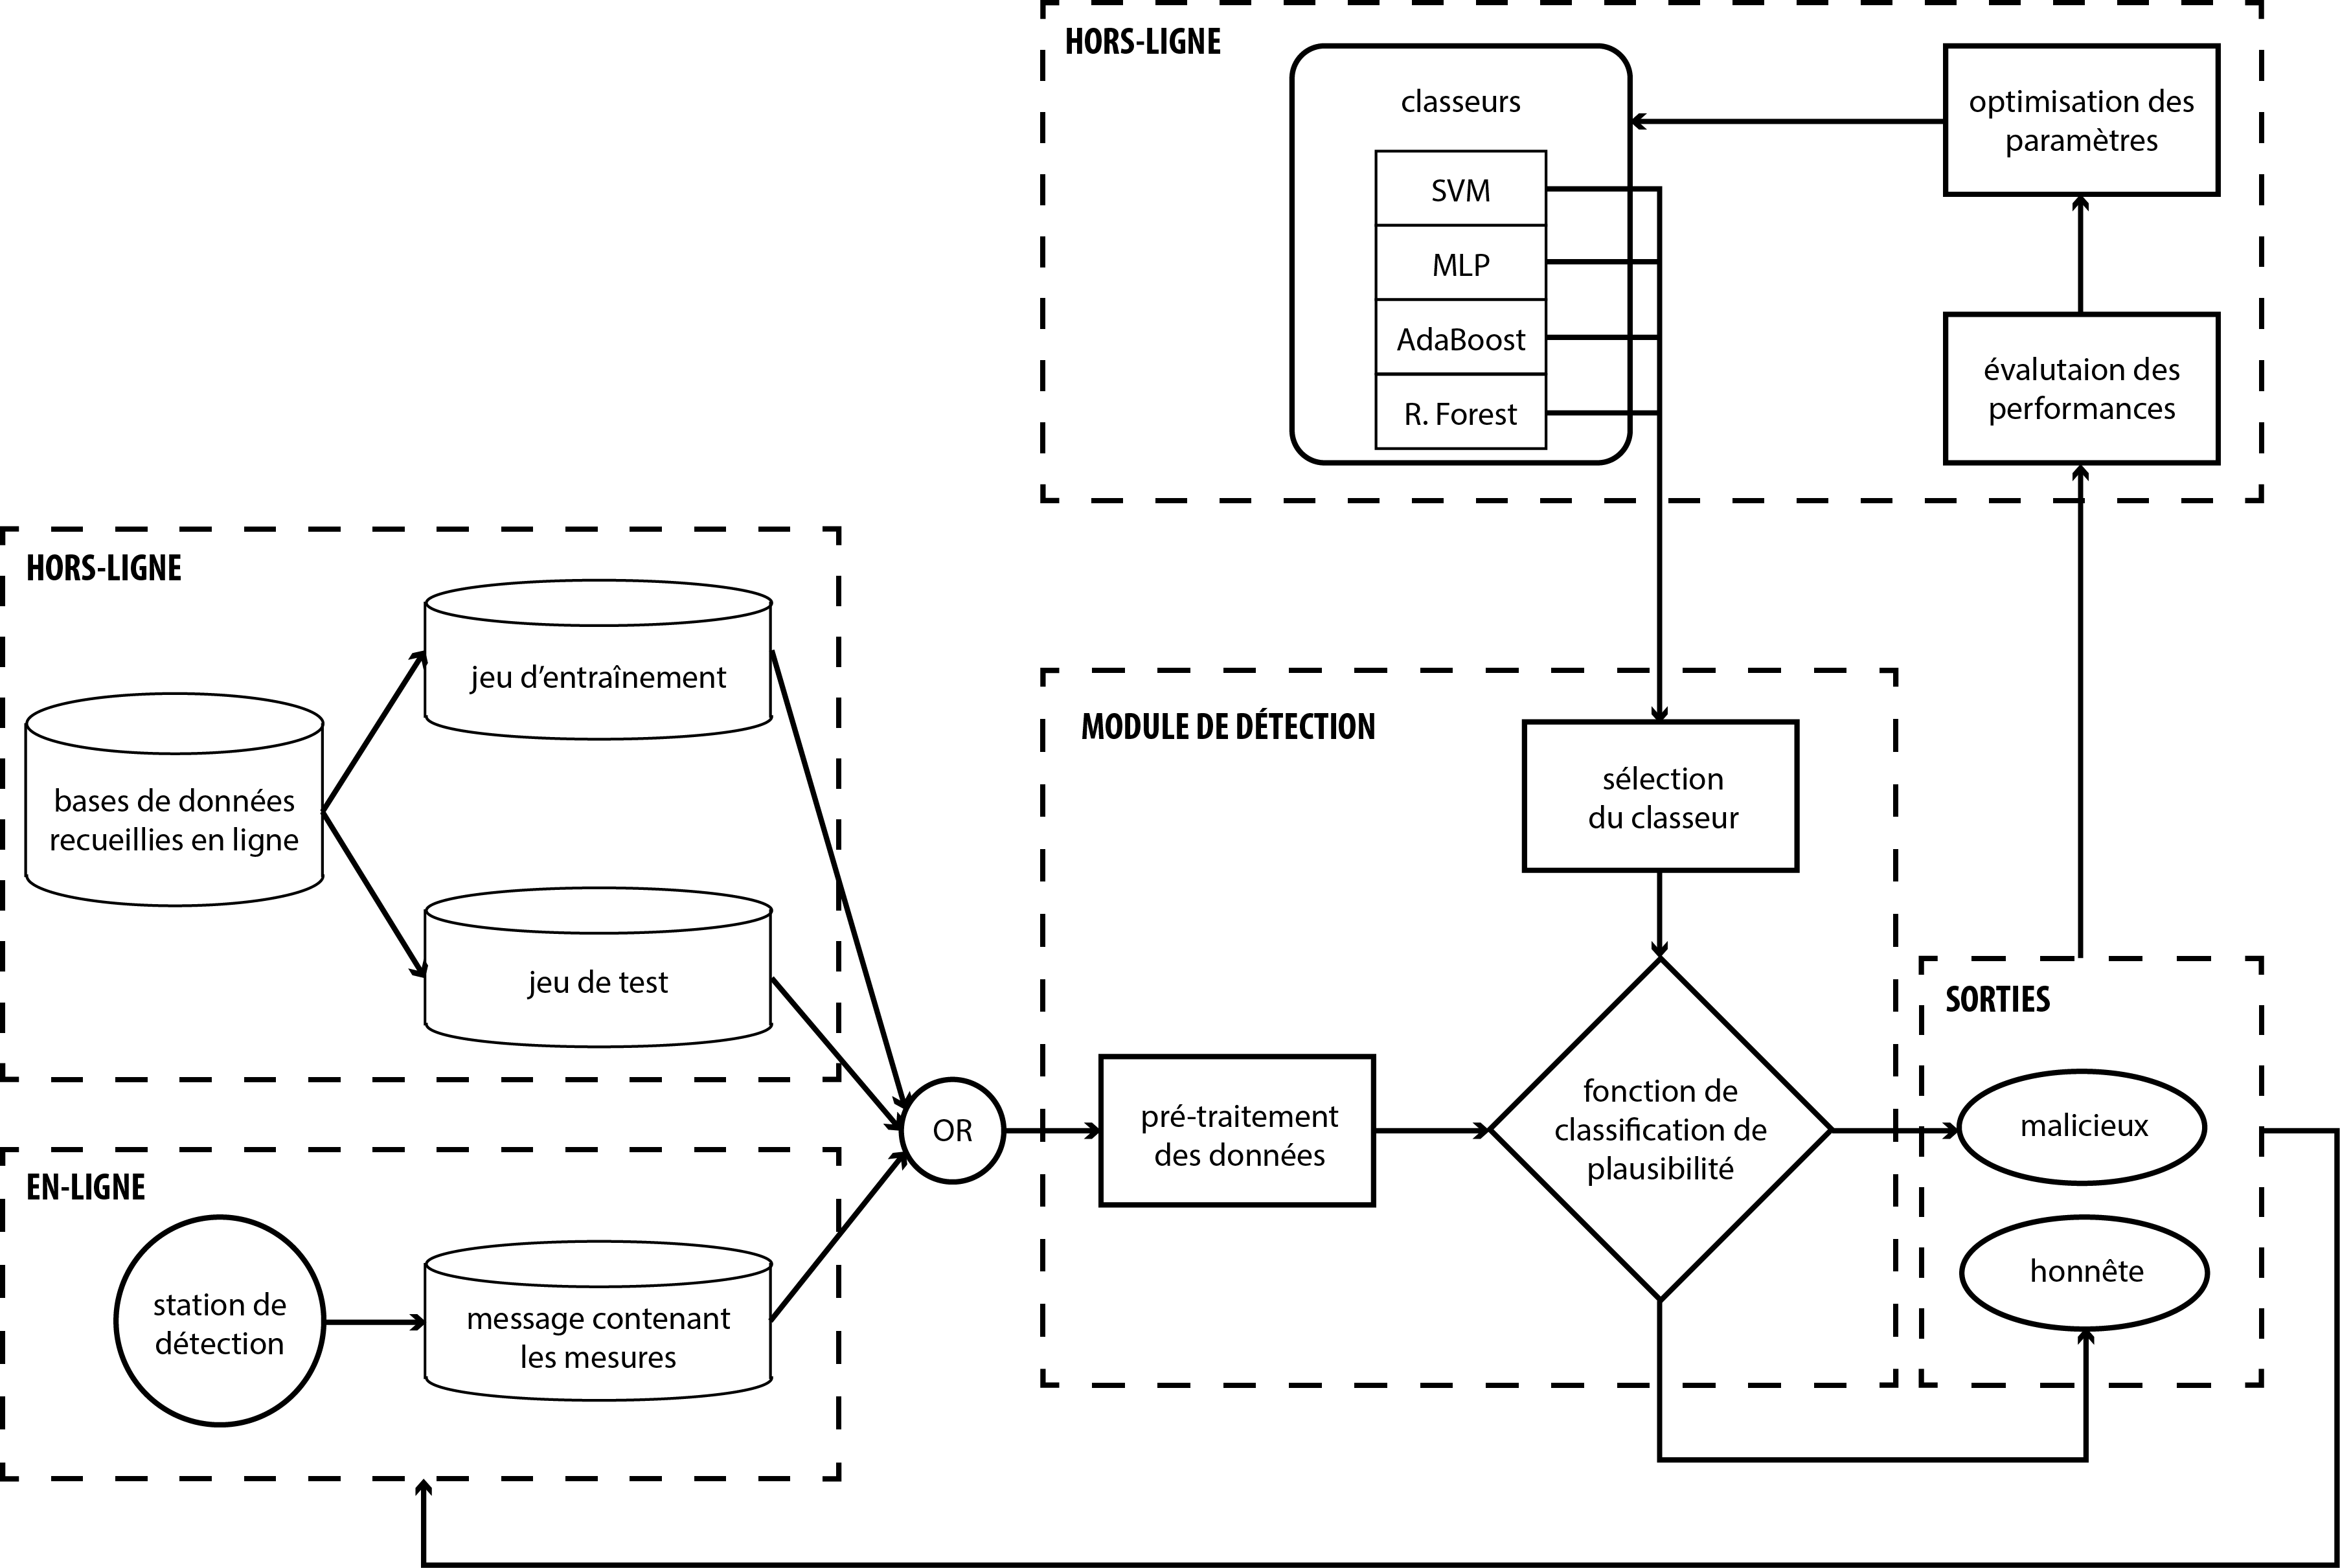
\includegraphics[width=\textwidth]{img/structure.png}
\caption{Schématisation du fonctionnement global du détecteur}
\end{figure}


\bibliography{bibliographie}
\bibliographystyle{unsrt}

\listoffigures
\begingroup
\let\clearpage\relax
\listoftables
\endgroup

\appendix

\chapter{Figures complémentaires}

\begin{figure}
\centering
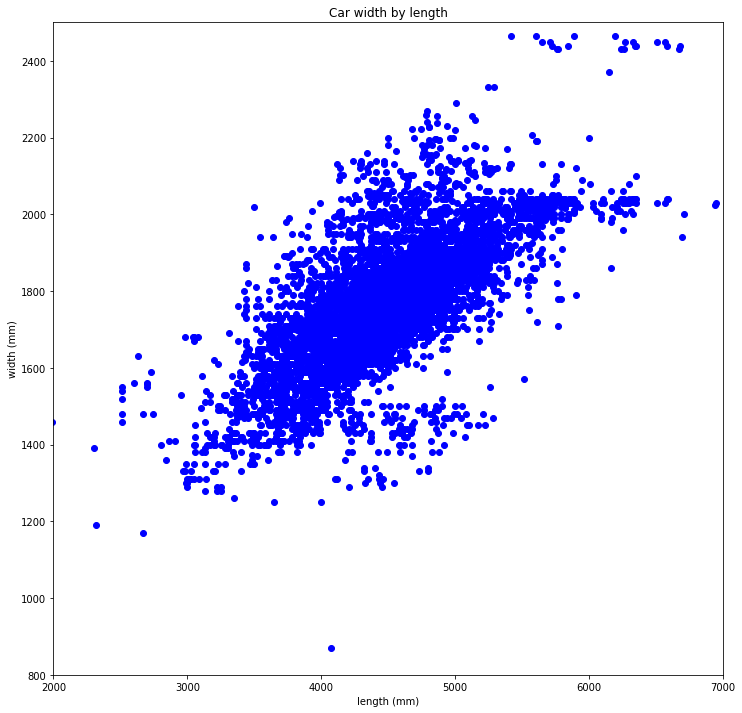
\includegraphics[width=\textwidth]{img/first_plot.png}
\caption{Premier affichage des données\label{first_plot}}
\end{figure}

\end{document}
